\chapter{JUSTIFICATIVA}
\label{chap:JUSTIFICATIVA}

Nossa proposta de IPS é de Posicionamento Remoto localizando dentro de um
ambiente fechado dispositivos conectados a internet (IoT Devices) através de
redes Wi-Fi e Bluetooth. Mediremos a distância destes MUs (devices) aos RP
(sensores) utilizando o resíduo eletromagnético das redes sem fio
(\textit{sniffing}) disponibilizando as informações encontradas através de uma
REST WEB API.

Sobre o contexto encontrado, propomos um ambiente consciente onde o contexto
locativo oriundo do posicionamento remoto de cada dispositivo móvel é
administrado e divulgado pelo prédio conectado ao invés da auto localização do
aparelho, pois:

\begin{alineas}

	\item Uma vez encontrada a localização, é mais fácil propagar esta informação do
ambiente para o aparelho em comparação ao auto posicionamento, pois a negociação
entre o ambiente e o aparelho é nula quando o primeiro contém a informação- o
ambiente sempre disponibilizará uma informação coletada para o gerador desta
informação;

	\item Pode-se lidar com grande heterogeneidade de dispositivos, uma vez
que cada um deles não precisa se adaptar para cada mudança de ambiente;

	\item Este tipo de informação já é contida nos históricos de cada Ponto de
	Acesso Wi-Fi (AP - \textit{Access Point}), porém:

	\begin{alineas}

		\item Geralmente sem uso - poucas são as aplicações que usam a
		localização obtida pelo AP;

		\item Com granularidade insuficiente para uso em aplicações
		contextualizadas;

		\item geralmente não disponibilizada pelos APs.

	\end{alineas}

	\item Uma vez instalado um PS deste gênero, a quantia de dispositivos que
	ele pode localizar fica limitada apenas pela rede física;

	\item Economia de hardware quando menos é exigido de cada dispositivo.

\end{alineas}

Levamos em conta também a quantidade prevista de em média 5 dispositivos IoT
por pessoa que seriam beneficiados sempre que utilizados no ambiente conectado.

\begin{figure}[htb]
	\caption{\label{fig:projeto}Modelo das camadas }
	\begin{center}
		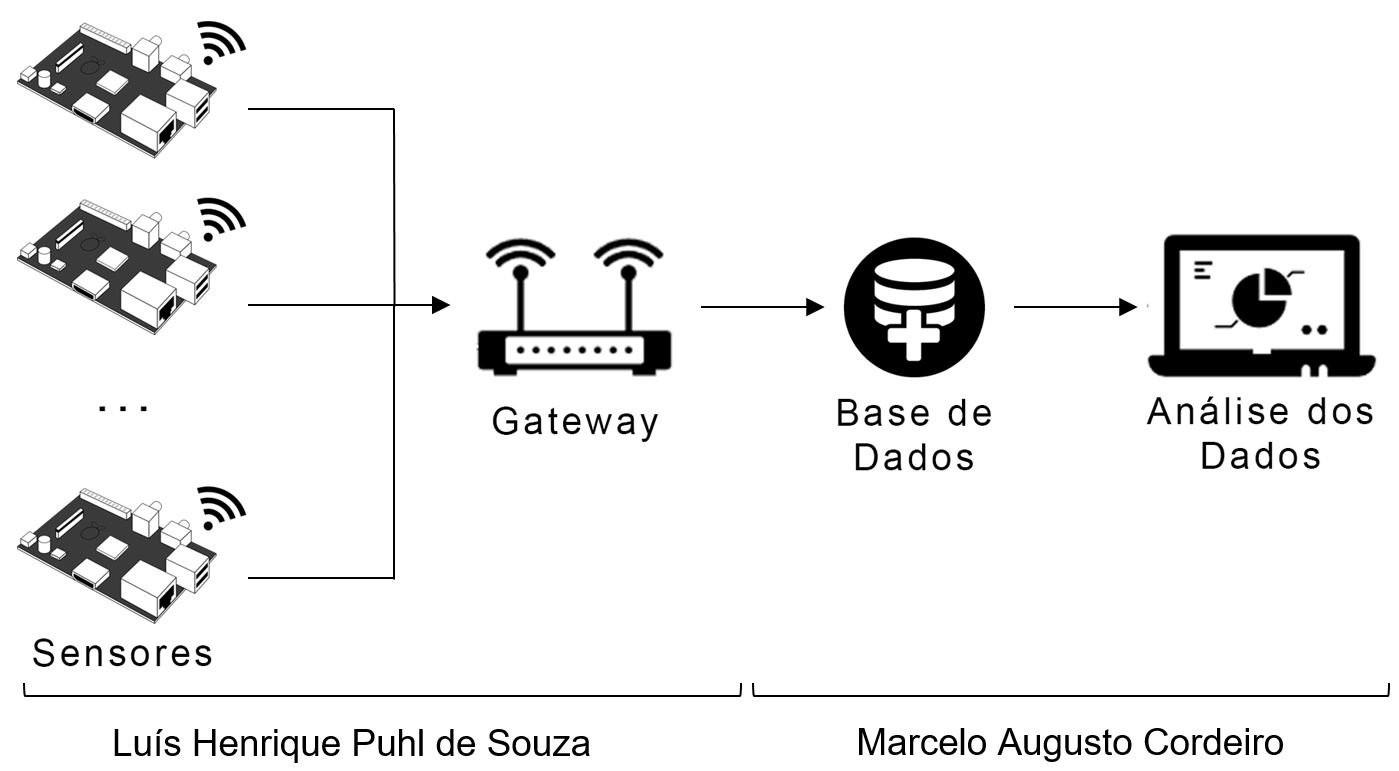
\includegraphics[width=1\textwidth]{img/projeto.JPG}
	\end{center}
	\legend{Fonte: Marcelo Augusto Cordeiro}
\end{figure}

A Figura \ref{fig:projeto} apresenta a arquitetura simplificada de uma aplicação
IoT.

Para possibilitar testes em um ambiente real, o projeto aqui proposto será
instalado dentro do prédio do Laboratório de Tecnologia da Informação Aplicada
(LTIA) da Faculdade de Ciências da Unesp de Bauru.
